\chapter{Introduction}

\label{chap:introduction}

\begin{figure}[t]
    \centering
    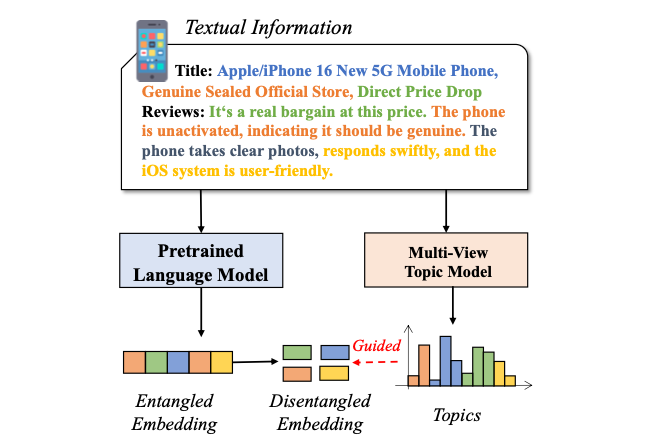
\includegraphics[width=0.9\linewidth]{Figures/Chapter1/figure1.png}
    \caption{Illustration of semantic embedding disentanglement.}
    \label{fig:disentangle}
\end{figure}

\section{Background and Motivation}

In the modern digital landscape, individuals are inundated with a virtually infinite amount of information. Whether shopping on e-commerce platforms like Amazon, streaming content on Netflix, or browsing news feeds on social media, users rely on recommendation systems to navigate this vast sea of choices. These systems act as personalized guides, curating content and products to match individual tastes and needs. This personalization is not merely a convenience; it is a critical driver of user experience, engagement, and, ultimately, platform revenue. A successful recommendation can delight a user and foster loyalty, while a poor one can lead to frustration and churn.\cite{El-Abidin2023Retention}

At the heart of this personalization engine lies a fundamental question: "Of all the items we could show a user, which one are they most likely to interact with?" In the digital world, the most common and measurable form of interaction is a click. Therefore, the ability to accurately estimate the probability of a user clicking on a specific item becomes a cornerstone technology. This task is formally known as Click-Through Rate (CTR) prediction. Due to its central role in optimizing user engagement and economic outcomes, CTR prediction has garnered immense attention from both industry practitioners and academic researchers~\cite{chen2016deep, zhou2018deep}.

Conventional CTR prediction methods typically comprise four main layers: the input layer, embedding layer, interaction layer, and prediction layer~\cite{guo2017deepfm, wang2021dcn}. The input layer incorporates a variety of features, including user attributes (e.g., gender, age, occupation, behavior sequences), item characteristics (e.g., category, brand), and contextual information (e.g., interaction location, time). These features are initially processed through the embedding layer to obtain feature embeddings. Subsequently, feature interaction layers, such as Factorization Machines~\cite{rendle2010factorization}, EulerNet~\cite{tian2023eulernet}, or KAN~\cite{shi2024beyond}, conduct interactions on the feature embeddings. The resulting interacted features are then fed into the prediction layer to estimate the final click probability.

Traditional CTR models primarily rely on structured categorical and numerical features~\cite{guo2021dual, liu2020autofis}. However, with the rapid advancement of Pretrained Language Models (PLMs)~\cite{devlin2019bert}, researchers have begun incorporating textual information to enrich semantic understanding and improve prediction accuracy~\cite{wang2023bert4ctr, chen2023tbin}. For instance, CTRL~\cite{li2023ctrl} collects textual descriptions of features and encodes them using PLMs to derive semantic embeddings. It employs a contrastive learning strategy to align collaborative signals with these semantic embeddings. 

Despite the effectiveness of PLMs in extracting semantic features, existing methods typically encode all textual information into a single dense embedding~\cite{liu2020category, yang2019learning}. As illustrated in Figure~\ref{fig:disentangle}, since textual descriptions inherently contain multiple aspects—such as brand, price, quality, and user sentiment—compressing them into a single representation leads to an entangled embedding. This entanglement hinders fine-grained feature interactions, limiting the model's ability to distinguish between different aspects of user preferences~\cite{ma2019learning, wang2020disentangled}.

For instance, consider a user browsing for a laptop. The product's title, 'BrandX Pro Laptop, 15-inch, High-Performance CPU, Lightweight for Business, On Sale', contains multiple semantic facets: brand ('BrandX'), specifications ('15-inch', 'High-Performance CPU'), usage scenario ('Business'), and promotion ('On Sale'). A user might click because they trust the brand, while another might be attracted by the sale price. An entangled embedding merges these distinct signals, making it difficult for the model to learn whether the user's core interest lies in 'BrandX', 'high performance', or 'discounted items'. This ambiguity can lead to suboptimal recommendations, such as pushing full-priced BrandX items to a price-sensitive user.

\section{Problem Statement and Challenges}

The fundamental challenge in text-enhanced CTR prediction lies in the effective utilization of multi-faceted textual information. Current approaches suffer from several limitations:

\textbf{Entangled Semantic Representations:} Existing methods~\cite{li2023ctrl, wang2023bert4ctr} typically encode entire textual descriptions into single dense vectors, which conflates distinct semantic aspects such as product features, brand information, user sentiment, and contextual descriptions. This entanglement prevents models from capturing nuanced user preferences and fine-grained feature interactions.

\textbf{Insufficient Semantic Disentanglement:} While disentangled representation learning has shown promise in recommendation systems~\cite{ma2019learning, wang2021multimodal, cao2022disencdr}, most approaches focus on collaborative filtering scenarios rather than CTR prediction with rich textual content. The challenge of extracting and separating meaningful semantic aspects from unstructured text remains largely unaddressed.

\textbf{Limited Integration of Multi-faceted Knowledge:} Even when different aspects of textual information can be identified, effectively incorporating them into CTR prediction models while maintaining their distinctiveness poses significant challenges~\cite{zhang2024towards}.

Addressing these issues presents two major challenges: 
\begin{enumerate}
    \item \textbf{Semantic Disentanglement Challenge:} How can we effectively disentangle and extract meaningful knowledge from textual information? Text descriptions contain rich but interwoven semantic aspects, making it challenging to separate distinct information (e.g., product features, user sentiment, and brand identity) and filter out noise~\cite{wang2024disentangled, locatello2019challenging}.
    \item \textbf{Knowledge Integration Challenge:} How can we effectively integrate multi-faceted knowledge into the CTR prediction task to extract useful information? Not all extracted textual information is relevant to user decision-making, so aligning it with CTR prediction is crucial for performance improvement~\cite{ni2019justifying, wong2021improving}.
\end{enumerate}

Successfully addressing these challenges would not only lead to significant improvements in CTR prediction accuracy but also unlock new possibilities for recommendation systems. A model capable of understanding disentangled user preferences could provide more diverse and personalized recommendations. For example, it could differentiate between a user's long-term interest in a brand and their short-term need for a specific product feature. Furthermore, the disentangled representations offer enhanced model interpretability, allowing researchers and practitioners to understand why a user clicked, thus enabling more transparent and controllable recommendation strategies.

\section{Proposed Approach}

To address these challenges, we propose \textbf{Multi-faceted Semantic Disentanglement for CTR prediction (MSD-CTR)}. Our approach draws inspiration from recent advances in disentangled representation learning~\cite{higgins2017beta, burgess2018understanding} and neural topic modeling~\cite{dieng2020topic, srivastava2017autoencoding} to create a unified framework for text-enhanced CTR prediction.

MSD-CTR consists of two key components: 

\begin{itemize}
    \item \textbf{Disentangled Semantic Topic Model (DSTopic):} This component employs a disentangled generative process to capture different aspects of documents using a Disentangled Semantic VAE (DSVAE) and a vocabulary clustering module. DSTopic builds upon recent advances in neural topic modeling~\cite{dieng2020topic, wu2023effective} while incorporating disentanglement principles from variational autoencoders~\cite{kingma2013auto, higgins2017beta}.
    
    \item \textbf{Topic Guided Disentangled Representation Learning (TopicDRL):} This component incorporates the multi-faceted knowledge into CTR prediction, introducing an individual-level alignment loss and an intra-view contrastive loss to guide semantic embedding learning. The design is motivated by recent work in contrastive learning for recommendation~\cite{lin2022feature} and causal disentanglement~\cite{yang2021causalvae, zheng2021disentangling}.
\end{itemize}

Unlike previous works\cite{li2023ctrl,kingma2013auto,higgins2017beta}, that either focus on disentangling collaborative signals or apply generic text encoders, MSD-CTR creates a synergistic bridge between neural topic modeling and CTR prediction. The core innovation lies in its ability to first explicitly model textual information as a distribution over disentangled semantic topics (via DSTopic) and then use this structured knowledge to guide the learning of user and item representations within the CTR framework (via TopicDRL). This two-stage process ensures that the disentangled knowledge is both meaningful and directly relevant to the prediction task.

\section{Contributions and Evaluation}

To evaluate the performance of MSD-CTR, we conduct extensive experiments on four real-world datasets and implement our model based on two foundational CTR methods~\cite{guo2017deepfm, wang2021dcn}. The results demonstrate that MSD-CTR outperforms existing CTR models~\cite{zhou2019deep, feng2019deep}. Additionally, we perform ablation studies and qualitative analyses to validate the effectiveness of the proposed components.

Our approach addresses the limitations of current text-enhanced CTR prediction methods by providing a principled way to disentangle semantic representations while maintaining their relevance to click prediction tasks. The integration of topic modeling with disentangled representation learning offers a novel perspective on handling multi-faceted textual information in recommendation scenarios.

\textbf{Our contributions can be summarized as follows:}
\begin{enumerate}
    \item We investigate text-enhanced CTR methods and analyze the issue of entangled semantic embeddings, providing both theoretical analysis and empirical evidence of the limitations in current approaches.
    \item We propose MSD-CTR, a novel framework that disentangles and incorporates multi-faceted knowledge from textual information via DSTopic and TopicDRL modules, bridging the gap between neural topic modeling and CTR prediction.
    \item We develop innovative loss functions including individual-level alignment loss and intra-view contrastive loss that effectively guide the learning of disentangled semantic representations for CTR tasks.
    \item We conduct extensive experiments demonstrating the superior performance of MSD-CTR across multiple datasets and baseline methods, along with comprehensive ablation studies that validate the contributions of individual components.
    \item We provide detailed qualitative analysis showing how our disentangled representations capture distinct semantic aspects, offering interpretability benefits alongside performance improvements.
\end{enumerate}

\section{Thesis Organization}

The remainder of this thesis is organized as follows: Chapter 2 reviews related work in CTR prediction, disentangled representation learning, and neural topic modeling. Chapter 3 presents the detailed methodology of our MSD-CTR framework. Chapter 4 describes our experimental setup and presents comprehensive results. Chapter 5 provides ablation studies and qualitative analysis. Finally, Chapter 6 concludes the thesis and discusses future research directions.